\state{Connection coefficients for spherical polar coordinates~(MCP 24.9)}{\hfix}

\prob{ \label{1a}
	Consider spherical polar coordinates in 3-dimensional space, and verify that the nonzero connection coefficients, assuming an orthonormal basis, are given by Eq.~(11.71).
}

\sol{
	We follow the procedure on pp.~1171--1172 of MCP for computing the connection coefficients.  We first evaluate the commutation coefficients $\csabsr$ using MCP~(24.38a),
	\eqn{commcoeff}{
		\csabsr = \ver \cdot [ \vesa, \vesb ],
	}
	We lower the last index using (24.38b),
	\eq{
		\csabg = \csabsr \sgsrg.
	}
	Then we use (24.38c) to compute
	\eqn{Gamthing}{
		\Gamsabg = \frac{1}{2} (\sgsabdg + \sgsagdb - \sgsbgda + \csabg + \csagb - \csbga),
	}
	and raise the first index using (24.38d),
	\eqn{Gamraise}{
		\Gammsbg = \sgma \Gamsabg.
	}
	From (24.40), the commutator is given by
	\eqn{comm}{
		[ \vA, \vB ] = \nabsvA \vB - \nabsvB \vA.
	}
	We also note that $\sgsab = \vesa \cdot \vesb$~\cite[p.~1161]{MCP}.
	
	For an orthonormal basis $\{ \rh, \thh, \phh \}$, $\sg$ is the Kronecker delta~\cite[p.~614]{MCP}.  In spherical coordinates, the gradient is
	\eq{
		\grad = \rh \pdv{r} + \frac{1}{r} \thh \pdv{\tht} + \frac{1}{r \sin\tht} \phh \pdv{\phi},
	}
	and its components are~\cite{Spherical}
	\al{
		\nabsr \rh &= \bo, &
		\nabst \rh &= \frac{1}{r} \thh, &
		\nabsp \rh &= \frac{1}{r} \phh, \\
		\nabsr \thh &= \bo, &
		\nabst \thh &= -\frac{1}{r} \rh, &
		\nabsp \thh &= \frac{1}{r \tan\tht} \phh, \\
		\nabsr \phh &= \bo, &
		\nabst \phh &= \bo, &
		\nabsp \phh &= -\frac{1}{r \tan\tht} \thh - \frac{1}{r} \rh.
	}
	Applying Eq.~\refeq{comm} and the above, we find
	\al{
		[ \rh, \rh ] &= \nabsr \rh - \nabsr \rh = \bo, &
		[ \rh, \thh ] &= \nabsr \thh - \nabst \rh = -\frac{1}{r} \thh, &
		[ \rh, \phh ] &= \nabsr \phh - \nabsp \rh = -\frac{1}{r} \phh, \\
		%
		[ \thh, \rh ] &= -[ \rh, \thh] = \frac{1}{r} \thh, &
		[ \thh, \thh ] &= \nabst \thh - \nabst \thh = \bo, &
		[ \thh, \phh ] &= \nabst \phh - \nabsp \thh = -\frac{1}{r \tan\tht} \phh, \\
		%
		[ \phh, \rh ] &= -[ \rh, \phh ] = \frac{1}{r} \phh, &
		[ \phh, \thh ] &= -[ \thh, \phh ] = \frac{1}{r \tan\tht} \phh, &
		[ \phh, \phh ] &= \nabsp \phh - \nabsp \phh = \bo.
	}
	Since $\sg$ is the Kronecker delta, we can immediately write from Eq.~\refeq{commcoeff}
	\al{
		c_{r r r} &= [ \rh, \rh ] \vdot \rh = 0, &
		c_{r \tht r} &= [ \rh, \thh ] \vdot \rh = 0, &
		c_{r \phi r} &= [ \rh, \phh ] \vdot \rh = 0, \\
		%
		c_{\tht r r} &= -c_{r \tht r} = 0, &
		c_{\tht \tht r} &= [ \thh, \thh ] \vdot \rh = 0, &
		c_{\tht \phi r} &= [ \thh, \phh ] \vdot \rh = 0, \\
		%
		c_{\phi r r} &= -c_{r \phi r} = 0, &
		c_{\phi \tht r} &= -c_{ \tht \phi r} = 0, &
		c_{\phi \phi r} &= [ \phh, \phh ] \vdot \rh = 0,
	}
	\al{
		c_{r r \tht} &= [ \rh, \rh ] \vdot \thh = 0, &
		c_{r \tht \tht} &= [ \rh, \thh ] \vdot \thh = -\frac{1}{r}, &
		c_{r \phi \tht} &= [ \rh, \phh ] \vdot \thh = 0, \\
		%
		c_{\tht r \tht} &= -c_{r \tht \tht} = \frac{1}{r}, &
		c_{\tht \tht \tht} &= [ \thh, \thh ] \vdot \thh = 0, &
		c_{\tht \phi \tht} &= [ \thh, \phh ] \vdot \thh = 0, \\
		%
		c_{\phi r \tht} &= -c_{r \phi \tht} = 0, &
		c_{\phi \tht \tht} &= -c_{\tht \phi \tht} = 0, &
		c_{\phi \phi \tht} &= [ \phh, \phh ] \vdot \thh = 0, \\[2ex]
		%
		%
		c_{r r \phi} &= [ \rh, \rh ] \vdot \phh = 0, &
		c_{r \tht \phi} &= [ \rh, \thh ] \vdot \phh = 0, &
		c_{r \phi \phi} &= [ \rh, \phh ] \vdot \phh = -\frac{1}{r}, \\
		%
		c_{\tht r \phi} &= -c_{r \tht \phi} = 0, &
		c_{\tht \tht \phi} &= [ \thh, \thh ] \vdot \phh = 0, &
		c_{\tht \phi \phi} &= [ \thh, \phh ] \vdot \phh = -\frac{1}{r \tan\tht}, \\
		%
		c_{\phi r \phi} &= -c_{r \phi \phi} = \frac{1}{r}, &
		c_{\phi \tht \phi} &= -c_{\tht \phi \tht} = \frac{1}{r \tan\tht}, &
		c_{\phi \phi \phi} &= [ \phh, \phh ] \vdot \phh = 0.
	}
	From Eq.~\refeq{Gamthing} we again use the fact that $\sg$ is the identity to write
	\al{
		\Gam_{r r r} &= \frac{c_{r r r} + c_{r r r} - c_{r r r}}{2} = 0, &
		\Gam_{r r \tht} &= \frac{c_{r r \tht} + c_{r \tht r} - c_{r \tht r}}{2} = 0, &
		\Gam_{r r \phi} &= \frac{c_{r r \phi} + c_{r \phi r} - c_{r \phi r}}{2} = 0, \\
		%
		\Gam_{r \tht r} &= \frac{c_{r \tht r} + c_{r r \tht} - c_{\tht r r}}{2} = 0, &
		\Gam_{r \tht \tht} &= \frac{c_{r \tht \tht} + c_{r \tht \tht} - c_{\tht \tht r}}{2} = -\frac{1}{r}, &
		\Gam_{r \tht \phi} &= \frac{c_{r \tht \phi} + c_{r \phi \tht} - c_{\tht \phi r}}{2} = 0, \\
		%
		\Gam_{r \phi r} &= \frac{c_{r \phi r} + c_{r r \phi} - c_{\phi r r}}{2} = 0, &
		\Gam_{r \phi \tht} &= \frac{c_{r \phi \tht} + c_{r \tht \phi} - c_{\phi \tht r}}{2} = 0, &
		\Gam_{r \phi \phi} &= \frac{c_{r \phi \phi} + c_{r \phi \phi} - c_{\phi \phi r}}{2} = -\frac{1}{r}, \\[2ex]
		%
		%
		\Gam_{\tht r r} &= \frac{c_{\tht r r} + c_{\tht r r} - c_{r r \tht}}{2} = 0, &
		\Gam_{\tht r \tht} &= \frac{c_{\tht r \tht} + c_{\tht \tht r} - c_{r \tht \tht}}{2} = \frac{1}{r}, &
		\Gam_{\tht r \phi} &= \frac{c_{\tht r \phi} + c_{\tht \phi r} - c_{r \phi \tht}}{2} = 0, \\
		%
		\Gam_{\tht \tht r} &= \frac{c_{\tht \tht r} + c_{\tht r \tht} - c_{\tht r \tht}}{2} = 0, &
		\Gam_{\tht \tht \tht} &= \frac{c_{\tht \tht \tht} + c_{\tht \tht \tht} - c_{\tht \tht \tht}}{2} = 0, &
		\Gam_{\tht \tht \phi} &= \frac{c_{\tht \tht \phi} + c_{\tht \phi \tht} - c_{\tht \phi \tht}}{2} = 0, \\
		%
		\Gam_{\tht \phi r} &= \frac{c_{\tht \phi r} + c_{\tht r \phi} - c_{\phi r \tht}}{2} = 0, &
		\Gam_{\tht \phi \tht} &= \frac{c_{\tht \phi \tht} + c_{\tht \tht \phi} - c_{\phi \tht \tht}}{2} = 0, &
		\Gam_{\tht \phi \phi} &= \frac{c_{\tht \phi \phi} + c_{\tht \phi \phi} - c_{\phi \phi \tht}}{2} = -\frac{1}{r \tan\tht}, \\[2ex]
		%
		%
		\Gam_{\phi r r} &= \frac{c_{\phi r r} + c_{\phi r r} - c_{r r \phi}}{2} = 0, &
		\Gam_{\phi r \tht} &= \frac{c_{\phi r \tht} + c_{\phi \tht r} - c_{r \tht \phi}}{2} = 0, &
		\Gam_{\phi r \phi} &= \frac{c_{\phi r \phi} + c_{\phi \phi r} - c_{r \phi \phi}}{2} = \frac{1}{r}, \\
		%
		\Gam_{\phi \tht r} &= \frac{c_{\phi \tht r} + c_{\phi r \tht} - c_{\tht r \phi}}{2} = 0, &
		\Gam_{\phi \tht \tht} &= \frac{c_{\phi \tht \tht} + c_{\phi \tht \tht} - c_{\tht \tht \phi}}{2} = 0, &
		\Gam_{\phi \tht \phi} &= \frac{c_{\phi \tht \phi} + c_{\phi \phi \tht} - c_{\tht \phi \phi}}{2} = \frac{1}{r \tan\tht}, \\
		%
		\Gam_{\phi \phi r} &= \frac{c_{\phi \phi r} + c_{\phi r \phi} - c_{\phi r \phi}}{2} = 0, &
		\Gam_{\phi \phi \tht} &= \frac{c_{\phi \phi \tht} + c_{\phi \tht \phi} - c_{\phi \tht \phi}}{2} = 0, &
		\Gam_{\phi \phi \phi} &= \frac{c_{\phi \phi \phi} + c_{\phi \phi \phi} - c_{\phi \phi \phi}}{2} = 0.
	}
	In summary, we have the nonzero connection coefficients
	\ans{\al{
		\Gam_{r \tht \tht} = \Gam_{r \phi \phi} &= -\frac{1}{r}, &
		\Gam_{\tht r \tht} = \Gam_{\phi r \phi} &= \frac{1}{r}, &
		\Gam_{\tht \phi \phi} &= -\frac{1}{r \tan\tht}, &
		\Gam_{\phi \tht \phi} &= \frac{1}{r \tan\tht}.
	}}%
	This is in agreement with MCP~(11.71), which gives the nonzero connection coefficients as
	\al{
		\Gam_{\tht r \tht} = \Gam_{\phi r \phi} = -\Gam_{r \tht \tht} = -\Gam_{r \phi \phi} &= \frac{1}{r}, &
		\Gam_{\phi \tht \phi} = -\Gam_{\tht \phi \phi} &= \frac{\cot\tht}{r}. \qed
	}
	\vfix
}



\prob{ \label{1b}
	Repeat the exercise in \ref{1a} assuming a coordinate basis with
	\al{
		\besr &\equiv \pdv{r}, &
		\bestht &\equiv \pdv{\tht}, &
		\besphi &\equiv \pdv{\phi}.
	}
	\vfix
}

\sol{
	In a coordinate basis, it is always true that $[ \vesa, \vesb ] = 0$~\cite[p.~1168]{MCP}.  In this case, the nonzero elements of $\sg$ are~\cite{Spherical}
	\al{
		\sg_{r r} &= 1, &
		\sg_{\tht \tht} &= r^2, &
		\sg_{\phi \phi} &= r^2 \sin^2\tht,
	}
	\clearpage
	which implies
	\al{
		\sg^{r r} &= 1, &
		\sg^{\tht \tht} &= \frac{1}{r^2}, &
		\sg^{\phi \phi} &= \frac{1}{r^2 \sin^2\tht},
	}
	since the matrix of contravariant components of the metric is inverse to that of the covariant components~\cite[p.~1162]{MCP}.  The only nonzero derivatives are
	\al{
		\sg_{\tht \tht, r} &= 2r, &
		\sg_{\phi \phi, r} &= 2 r \sin^2\tht, &
		\sg_{\phi \phi, \tht} &= 2 r^2 \sin\tht \cos\tht.
	}
	From Eq.~\refeq{Gamthing}, the $\Gamsabg$ are
	\al{
		\Gam_{r r r} &= \frac{\sg_{r r, r} + \sg_{r r, r} - \sg_{r r, r}}{2} = 0, &
		\Gam_{r r \tht} &= \frac{\sg_{r r, \tht} + \sg_{r \tht, r} - \sg_{r \tht, r}}{2} = 0, \\
		\Gam_{r r \phi} &= \frac{\sg_{r r, \phi} + \sg_{r \phi, r} - \sg_{r \phi, r}}{2} = 0, &
		%
		\Gam_{r \tht r} &= \frac{\sg_{r \tht, r} + \sg_{r r, \tht} - \sg_{r r, \tht}}{2} = 0, \\
		\Gam_{r \tht \tht} &= \frac{\sg_{r \tht, \tht} + \sg_{r \tht, \tht} - \sg_{\tht \tht, r}}{2} = -r, &
		\Gam_{r \tht \phi} &= \frac{\sg_{r \tht, \phi} + \sg_{r \phi, \tht} - \sg_{\tht \phi, r}}{2} = 0, \\
		%
		\Gam_{r \phi r} &= \frac{\sg_{r \phi, r} + \sg_{r r, \phi} - \sg_{\phi r, r}}{2} = 0, &
		\Gam_{r \phi \tht} &= \frac{\sg_{r \phi, \tht} + \sg_{r \tht, \phi} - \sg_{\phi \tht, r}}{2} = 0, \\
		\Gam_{r \phi \phi} &= \frac{\sg_{r \phi, \phi} + \sg_{r \phi, \phi} - \sg_{\phi \phi, r}}{2} = -r \sin^2\tht, \\[2ex]
		%
		%
		\Gam_{\tht r r} &= \frac{\sg_{\tht r, r} + \sg_{\tht r, r} - \sg_{r r, \tht}}{2} = 0, &
		\Gam_{\tht r \tht} &= \frac{\sg_{\tht r, \tht} + \sg_{\tht \tht, r} - \sg_{r \tht, \tht}}{2} = r, \\
		\Gam_{\tht r \phi} &= \frac{\sg_{\tht r, \phi} + \sg_{\tht \phi, r} - \sg_{r \phi, \tht}}{2} = 0, &
		%
		\Gam_{\tht \tht r} &= \frac{\sg_{\tht \tht, r} + \sg_{\tht r, \tht} - \sg_{\tht r, \tht}}{2} = r, \\
		\Gam_{\tht \tht \tht} &= \frac{\sg_{\tht \tht, \tht} + \sg_{\tht \tht, \tht} - \sg_{\tht \tht, \tht}}{2} = 0, &
		\Gam_{\tht \tht \phi} &= \frac{\sg_{\tht \tht, \phi} + \sg_{\tht \phi, \tht} - \sg_{\tht \phi, \tht}}{2} = 0, \\
		%
		\Gam_{\tht \phi r} &= \frac{\sg_{\tht \phi, r} + \sg_{\tht r, \phi} - \sg_{\phi r, \tht}}{2} = 0, &
		\Gam_{\tht \phi \tht} &= \frac{\sg_{\tht \phi, \tht} + \sg_{\tht \tht, \phi} - \sg_{\phi \tht, \tht}}{2} = 0, \\
		\Gam_{\tht \phi \phi} &= \frac{\sg_{\tht \phi, \phi} + \sg_{\tht \phi, \phi} - \sg_{\phi \phi, \tht}}{2} = -r^2 \sin\tht \cos\tht, \\[2ex]
		%
		%
		\Gam_{\phi r r} &= \frac{\sg_{\phi r, r} + \sg_{\phi r, r} - \sg_{r r, \phi}}{2} = 0, &
		\Gam_{\phi r \tht} &= \frac{\sg_{\phi r, \tht} + \sg_{\phi \tht, r} - \sg_{r \tht, \phi}}{2} = 0, \\
		\Gam_{\phi r \phi} &= \frac{\sg_{\phi r, \phi} + \sg_{\phi \phi, r} - \sg_{r \phi, \phi}}{2} = r \sin^2\tht, &
		%
		\Gam_{\phi \tht r} &= \frac{\sg_{\phi \tht, r} + \sg_{\phi r, \tht} - \sg_{\tht r, \phi}}{2} = 0, \\
		\Gam_{\phi \tht \tht} &= \frac{\sg_{\phi \tht, \tht} + \sg_{\phi \tht, \tht} - \sg_{\tht \tht, \phi}}{2} = 0, &
		\Gam_{\phi \tht \phi} &= \frac{\sg_{\phi \tht, \phi} + \sg_{\phi \phi, \tht} - \sg_{\tht \phi, \phi}}{2} = r^2 \sin\tht \cos\tht, \\
		%
		\Gam_{\phi \phi r} &= \frac{\sg_{\phi \phi, r} + \sg_{\phi r, \phi} - \sg_{\phi r, \phi}}{2} = r \sin^2\tht, &
		\Gam_{\phi \phi \tht} &= \frac{\sg_{\phi \phi, \tht} + \sg_{\phi \tht, \phi} - \sg_{\phi \tht, \phi}}{2} = r^2 \sin\tht \cos\tht, \\
		\Gam_{\phi \phi \phi} &= \frac{\sg_{\phi \phi, \phi} + \sg_{\phi \phi, \phi} - \sg_{\phi \phi, \phi}}{2} = 0.
	}
	Now applying Eq.~\refeq{Gamraise},
	\al{
		\Gam^r{}_{r r} &= \sg^{r r} \Gam_{r r r} = 0, &
		\Gam^r{}_{r \tht} &= \sg^{r r} \Gam_{r r \tht} = 0, &
		\Gam^r{}_{r \phi} &= \sg^{r r} \Gam_{r r \phi} = 0, \\
		%
		\Gam^r{}_{\tht r} &= \sg^{r r} \Gam_{r \tht r} = 0, &
		\Gam^r{}_{\tht \tht} &= \sg^{r r} \Gam_{r \tht \tht} = -r, &
		\Gam^r{}_{\tht \phi} &= \sg^{r r} \Gam_{r \tht \phi} = 0, \\
		%
		\Gam^r{}_{\phi r} &= \sg^{r r} \Gam_{r \phi r} = 0, &
		\Gam^r{}_{\phi \tht} &= \sg^{r r} \Gam_{r \phi r} = 0, &
		\Gam^r{}_{\phi \phi} &= \sg^{r r} \Gam_{r \phi \phi} = -r\sin^2\tht, \\[2ex]
		%
		%
		\Gam^\tht{}_{r r} &= \sg^{\tht \tht} \Gam_{\tht r r} = 0, &
		\Gam^\tht{}_{r \tht} &= \sg^{\tht \tht} \Gam_{\tht r \tht} = \frac{1}{r}, &
		\Gam^\tht{}_{r \phi} &= \sg^{\tht \tht} \Gam_{\tht r \phi} = 0, \\
		%
		\Gam^\tht{}_{\tht r} &= \sg^{\tht \tht} \Gam_{\tht \tht r} = \frac{1}{r}, &
		\Gam^\tht{}_{\tht \tht} &= \sg^{\tht \tht} \Gam_{\tht \tht \tht} = 0, &
		\Gam^\tht{}_{\tht \phi} &= \sg^{\tht \tht} \Gam_{\tht \tht \phi} = 0, \\
		%
		\Gam^\tht{}_{\phi r} &= \sg^{\tht \tht} \Gam_{\tht \phi r} = 0, &
		\Gam^\tht{}_{\phi \tht} &= \sg^{\tht \tht} \Gam_{\tht \phi \tht} = 0, &
		\Gam^\tht{}_{\phi \phi} &= \sg^{\tht \tht} \Gam_{\tht \phi \phi} = -\sin\tht \cos\tht,
	}
	\al{
		\Gam^\phi{}_{r r} &= \sg^{\phi \phi} \Gam_{\phi r r} = 0, &
		\Gam^\phi{}_{r \tht} &= \sg^{\phi \phi} \Gam_{\phi r \tht} = 0, &
		\Gam^\phi{}_{r \phi} &= \sg^{\phi \phi} \Gam_{\phi r \phi} = \frac{1}{r}, \\
		%
		\Gam^\phi{}_{\tht r} &= \sg^{\phi \phi} \Gam_{\phi \tht r} = 0, &
		\Gam^\phi{}_{\tht \tht} &= \sg^{\phi \phi} \Gam_{\phi \tht \tht} = 0, &
		\Gam^\phi{}_{\tht \phi} &= \sg^{\phi \phi} \Gam_{\phi \tht \phi} = \frac{1}{\tan\tht}, \\
		%
		\Gam^\phi{}_{\phi r} &= \sg^{\phi \phi} \Gam_{\phi \phi r} = \frac{1}{r}, &
		\Gam^\phi{}_{\phi \tht} &= \sg^{\phi \phi} \Gam_{\phi \phi \tht} = \frac{1}{\tan\tht}, &
		\Gam^\phi{}_{\phi \phi} &= \sg^{\phi \phi} \Gam_{\phi \phi \phi} = 0.
	}
	Thus we have found that the nonzero connection coeffients are
	\ans{\al{
		\Gam^r{}_{\tht \tht} &= -r, &
		\Gam^r{}_{\phi \phi} &= -r\sin^2\tht, &
		\Gam^\tht{}_{\phi \phi} &= -\sin\tht \cos\tht, &
		\Gam^\phi{}_{\tht \phi} &= \Gam^\phi{}_{\phi \tht} = \frac{1}{\tan\tht},
	}
	\eq{
		\Gam^\tht{}_{r \tht} = \Gam^\tht{}_{\tht r} = \Gam^\phi{}_{r \phi} = \Gam^\phi{}_{\phi r} = \frac{1}{r}.
	}}%
	\vfix
}



\prob{
	Repeat both computations in \ref{1a} and \ref{1b} using symbolic manipulation software on a computer.
}

\sol{
	For \ref{1b}, we use the Mathematica notebook from Ref.~\cite{Hartle} with $r \to 1$, $\tht \to 2$, and $\phi \to 3$:
	
	\scalebox{0.625}{
		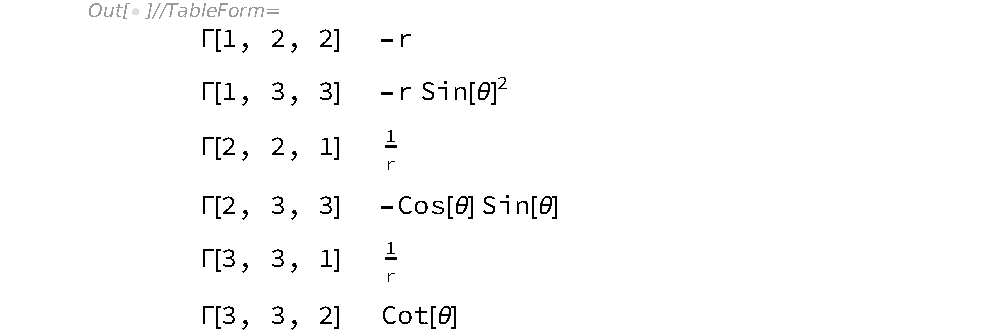
\includegraphics{1c-b}
	}
	
	Taking into account that in a coordinate basis $\Gamsabg$ is symmetric in its last two indices~\cite[p.~1172]{MCP}, these match our result from \ref{1b}.
	
	For \ref{1a}, I wrote a Mathematica notebook on my own (taking some inspiration from Ref.~\cite{Hartle}):
	
	\scalebox{0.625}{
		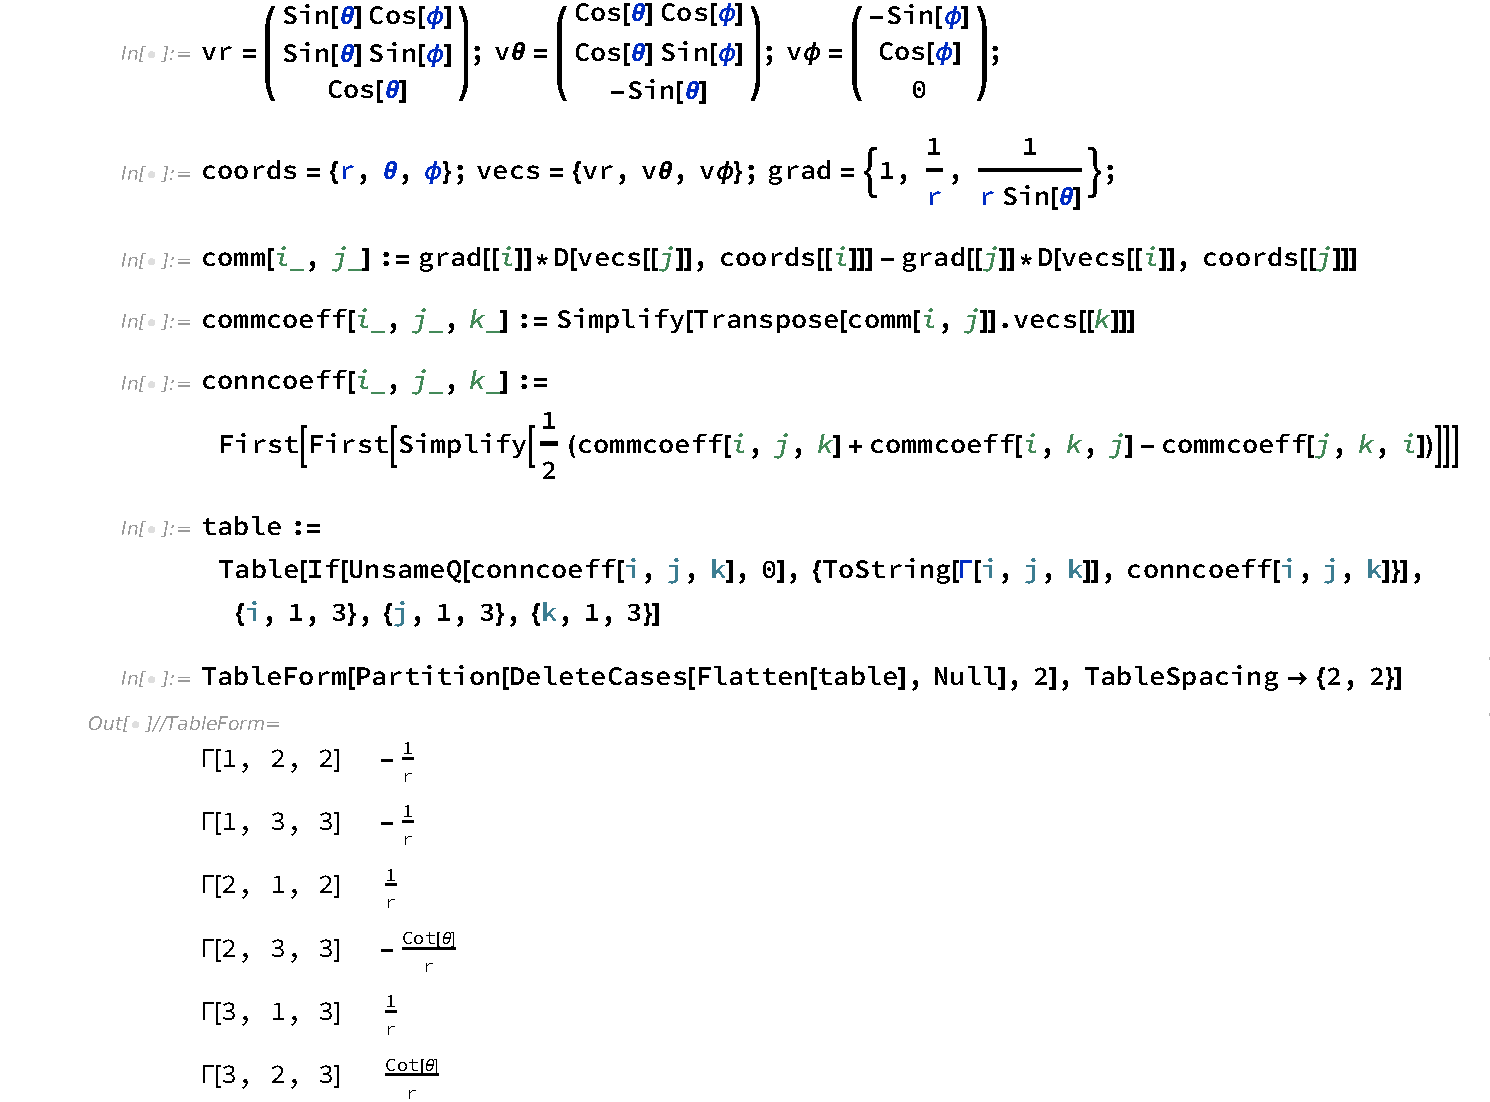
\includegraphics{1c-a}
	}
	
	For the result, we again have $r \to 1$, $\tht \to 2$, and $\phi \to 3$.  These match our result from \ref{1a}.
}